\documentclass[aps,prl,twocolumn,groupedaddress]{revtex4-1}
% \documentclass[aps,twocolumn,secnumarabic,balancelastpage,amsmath,amssymb,nofootinbib]{revtex4-1}
\usepackage{amsmath}
\usepackage{amssymb}
\usepackage{amsfonts}
\usepackage{color}
\usepackage{graphics}
\usepackage[pdftex]{graphicx}
\usepackage[utf8x]{inputenc}
\usepackage[colorlinks=true]{hyperref}

\newcommand{\ud}{\mathrm{d}}
\newcommand{\ue}{\mathrm{e}}
\newcommand{\ui}{\mathrm{i}}
\newcommand{\res}{\mathrm{Res}}
\newcommand{\Tr}{\mathrm{Tr}}
\newcommand{\dsum}{\displaystyle\sum}
\newcommand{\dprod}{\displaystyle\prod}
\newcommand{\dlim}{\displaystyle\lim}
\newcommand{\dint}{\displaystyle\int}
\newcommand{\fsno}[1]{{\!\not\!{#1}}}
\newcommand{\texp}[2]{\ensuremath{{#1}\times10^{#2}}}
\newcommand{\dexp}[2]{\ensuremath{{#1}\cdot10^{#2}}}
\newcommand{\eval}[2]{{\left.{#1}\right|_{#2}}}
\newcommand{\paren}[1]{{\left({#1}\right)}}
\newcommand{\lparen}[1]{{\left({#1}\right.}}
\newcommand{\rparen}[1]{{\left.{#1}\right)}}
\newcommand{\abs}[1]{{\left|{#1}\right|}}
\newcommand{\sqr}[1]{{\left[{#1}\right]}}
\newcommand{\crly}[1]{{\left\{{#1}\right\}}}
\newcommand{\angl}[1]{{\left\langle{#1}\right\rangle}}
\newcommand{\tpdiff}[4][{}]{{\paren{\frac{\partial^{#1} {#2}}{\partial {#3}{}^{#1}}}_{#4}}}
\newcommand{\tpsdiff}[4][{}]{{\paren{\frac{\partial^{#1}}{\partial {#3}{}^{#1}}{#2}}_{#4}}}
\newcommand{\pdiff}[3][{}]{{\frac{\partial^{#1} {#2}}{\partial {#3}{}^{#1}}}}
\newcommand{\diff}[3][{}]{{\frac{\ud^{#1} {#2}}{\ud {#3}{}^{#1}}}}
\newcommand{\psdiff}[3][{}]{{\frac{\partial^{#1}}{\partial {#3}{}^{#1}} {#2}}}
\newcommand{\sdiff}[3][{}]{{\frac{\ud^{#1}}{\ud {#3}{}^{#1}} {#2}}}
\newcommand{\tpddiff}[4][{}]{{\left(\dfrac{\partial^{#1} {#2}}{\partial {#3}{}^{#1}}\right)_{#4}}}
\newcommand{\tpsddiff}[4][{}]{{\paren{\dfrac{\partial^{#1}}{\partial {#3}{}^{#1}}{#2}}_{#4}}}
\newcommand{\pddiff}[3][{}]{{\dfrac{\partial^{#1} {#2}}{\partial {#3}{}^{#1}}}}
\newcommand{\ddiff}[3][{}]{{\dfrac{\ud^{#1} {#2}}{\ud {#3}{}^{#1}}}}
\newcommand{\psddiff}[3][{}]{{\frac{\partial^{#1}}{\partial{}^{#1} {#3}} {#2}}}
\newcommand{\sddiff}[3][{}]{{\frac{\ud^{#1}}{\ud {#3}{}^{#1}} {#2}}}
\newcommand{\eff}{ef\! f}
\newcommand{\fxnote}[1]{{\textbf{[#1]}}}

\begin{document}
\title{Motional Ground State Cooling Outside the Lamb-Dicke Regime}
\author{Yichao Yu}
\email{yichaoyu@g.harvard.edu}
\author{Nicholas R. Hutzler}
\altaffiliation{Present address: California Institute of Technology, Division of Physics, Mathematics, and Astronomy.  Pasadena, CA, 91125}
\author{Jessie T. Zhang}
\author{Lee R. Liu}
\author{Kang-Kuen Ni}
\email{ni@chemistry.harvard.edu}
\affiliation{Department of Chemistry and Chemical Biology, Harvard University, Cambridge, Massachusetts, 02138, USA}
\affiliation{Department of Physics, Harvard University, Cambridge, Massachusetts, 02138, USA}
\affiliation{Harvard-MIT Center for Ultracold Atoms, Cambridge, Massachusetts, 02138, USA}

\date{\today}

\begin{abstract}
  We report Raman sideband cooling of a single sodium atom to its three-dimensional
  motional ground state in an optical tweezer.
  Despite having a very large Lamb-Dicke parameter, high initial temperature, and
  large differential AC Stark shifts in the excited state,
  we achieve a ground state preparation fidelity of $77(4)$\% after $100$ ms of cooling.
  Our technique includes addressing very high-order sidebands and
  fast modulation of the optical tweezer trap.
  We demonstrate that Raman sideband cooling to the 3D motional ground state is applicable
  outside the Lamb-Dicke regime, for example in
  systems where tight confinement and low initial temperature are difficult to realize.
  This is particularly relevant for systems which are challenging to laser-cool,
  such as molecules and exotic atoms,
  and opens up the possibility to gain quantum motional control of these systems.
\end{abstract}

\maketitle

\begin{figure*}
  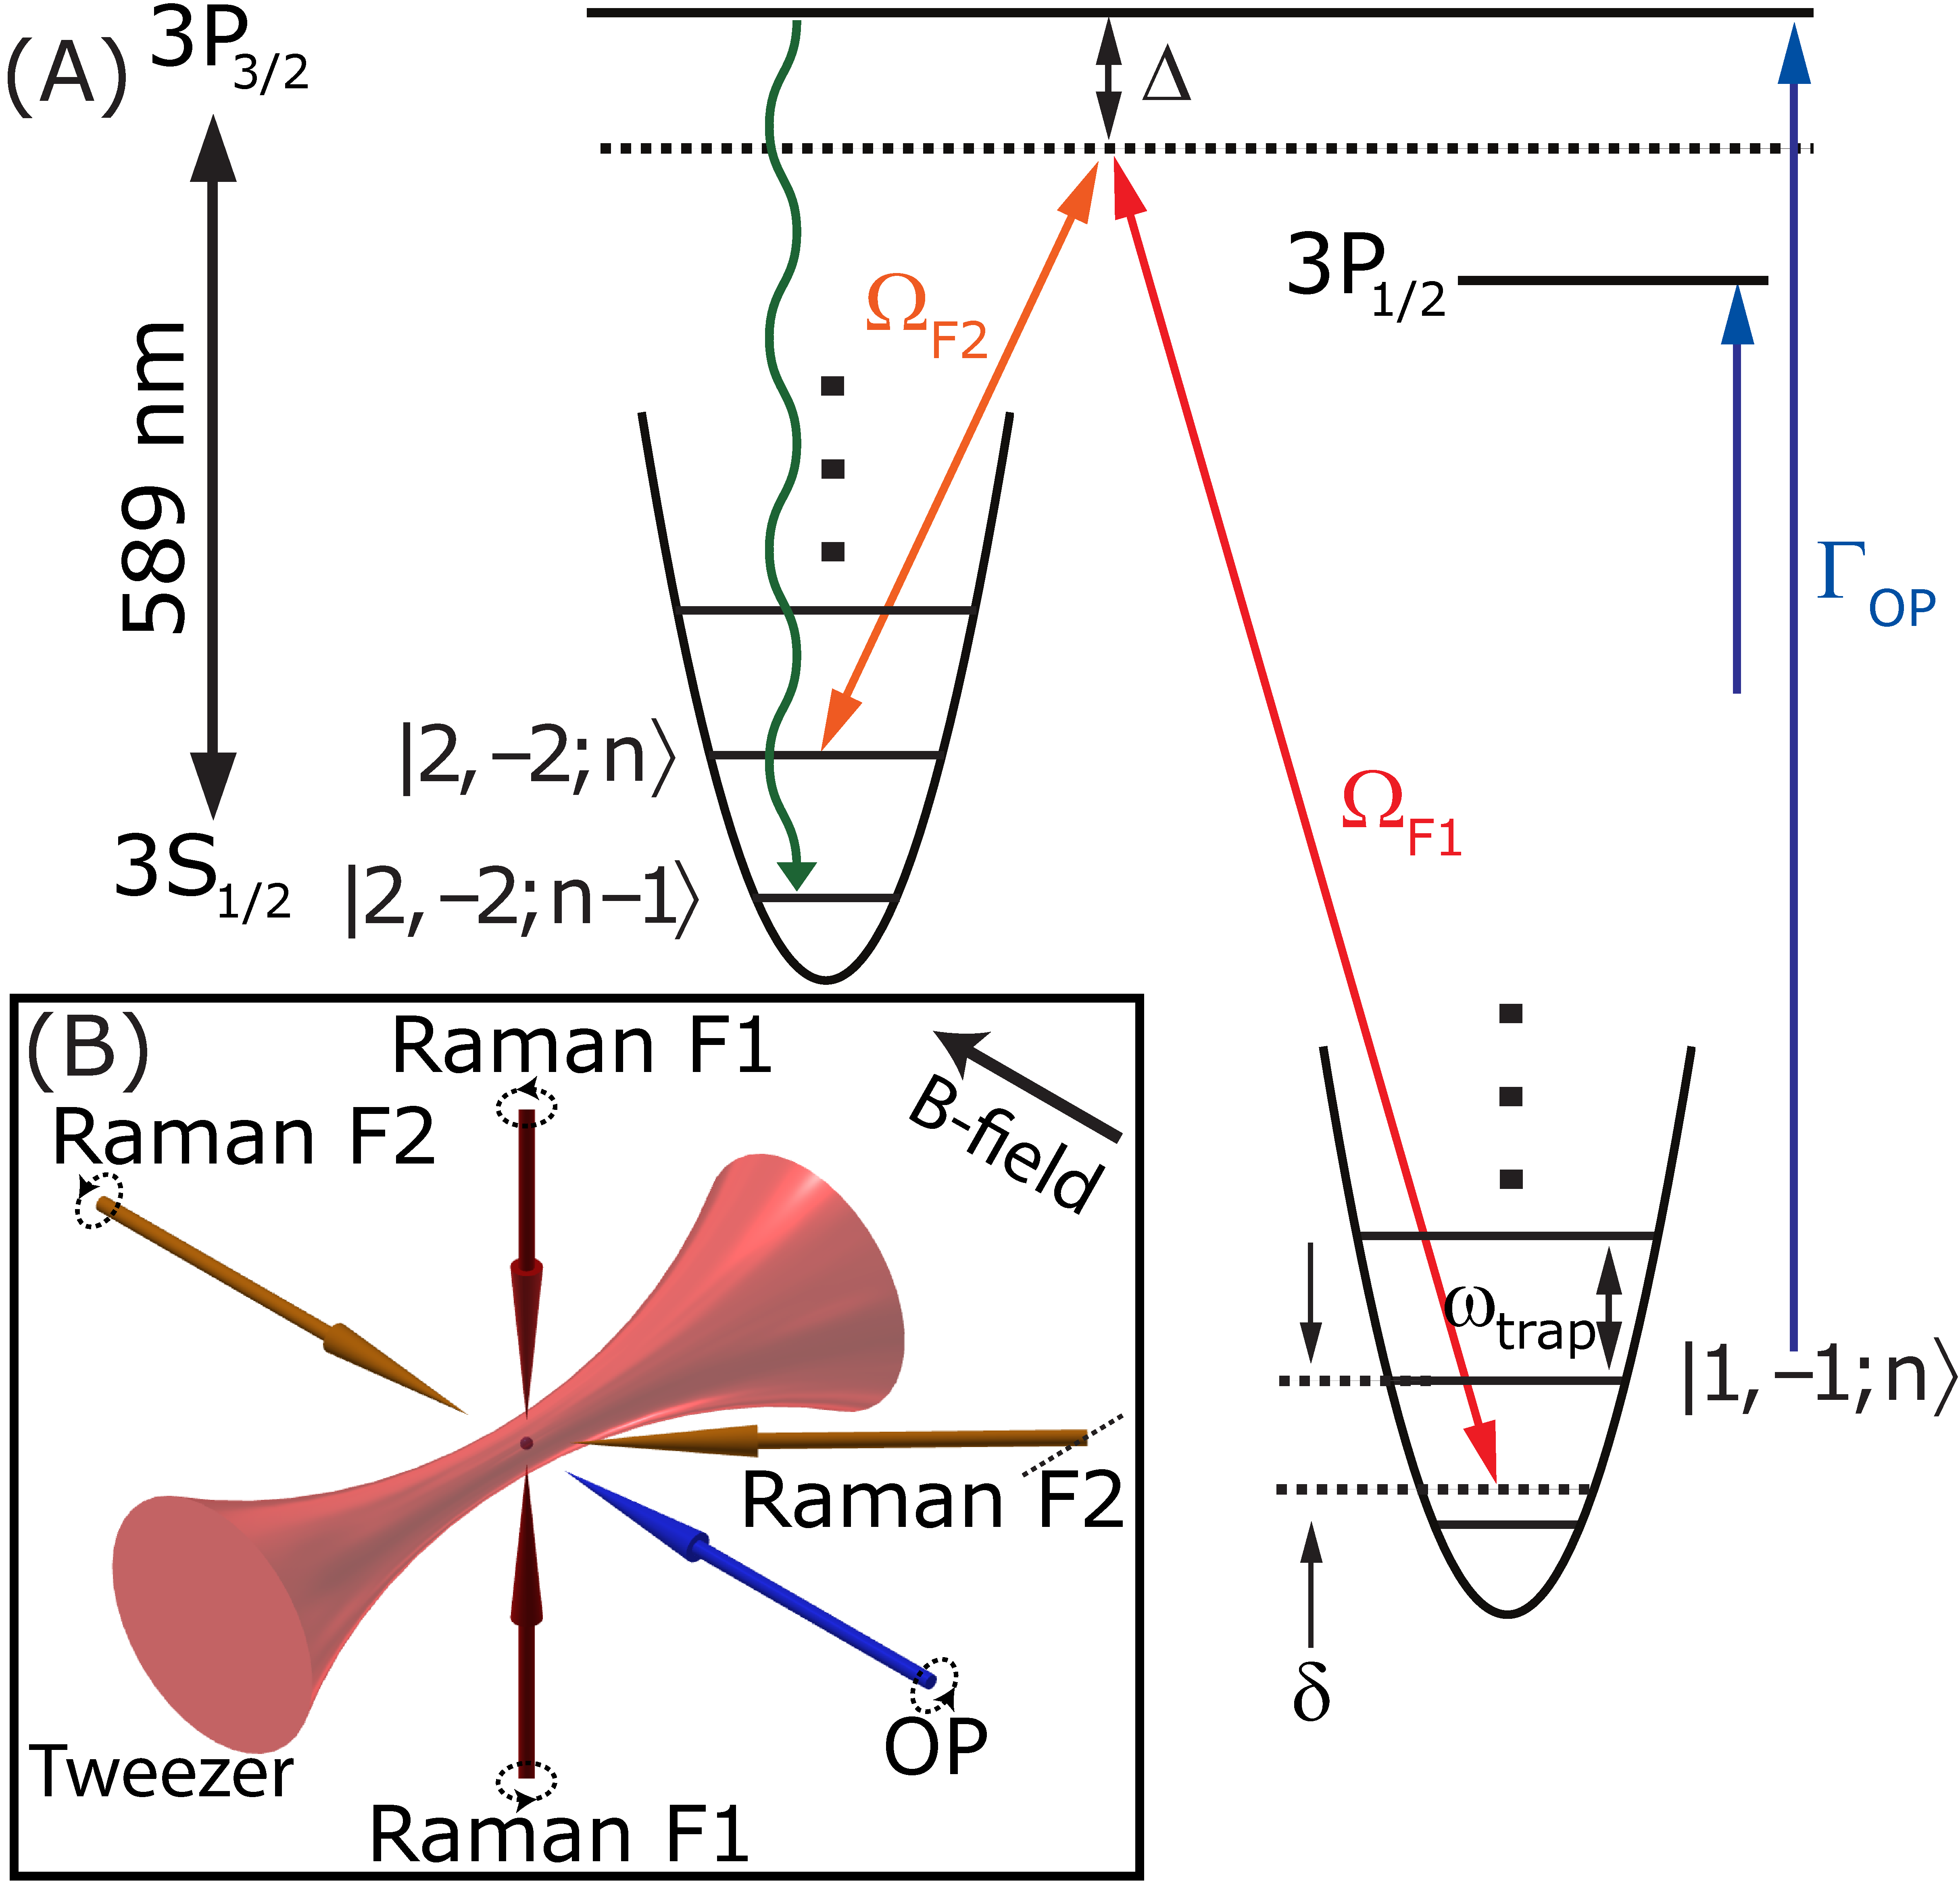
\includegraphics[height=5.2cm]{imgs/Na_RSC_schematic.pdf}
  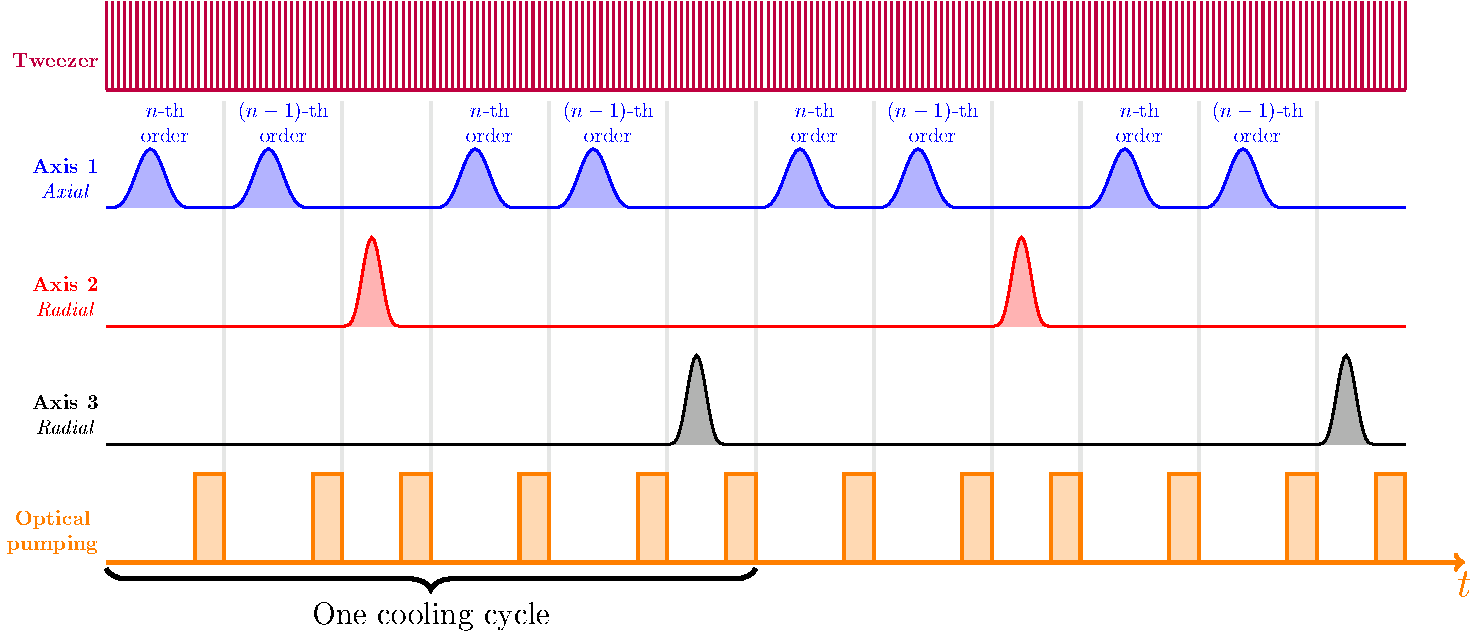
\includegraphics[height=4.5cm]{sequence.pdf}
  \caption{(A) Energy levels and schematic of Raman sideband cooling.
    The Raman transitions have a one photon detuning $\Delta=25$ GHz from the D2 line.
    We use D1 light with $\sigma^-$ polarization to repump atoms out of $|F=2,m_F=-1\rangle$
    state to minimize heating on the atom in the $|F=2,m_F=-2\rangle$ state
    (B) Geometry and polarizations of the Raman and optical pumping beams relative to the
    optical tweezer and bias magnetic field.
    (C) Schematic of the cooling sequence. The tweezer switches at 3 MHz to
    reduce light shifts during optical pumping. Each cooling cycle consists of $8$ pulses.
    The four axial pulses are addressing two neighboring cooling orders.
    The two pulses in each radial direction are either addressing two neighboring cooling orders
    or having different length on the first order when most of the population are below $n=3$
    towards the end of the cooling sequence.
    All of the Raman pulses use Blackman pulse envelopes to reduce the off-resonant
    coupling to carrier and heating sidebands.
    \label{f-setup}}
\end{figure*}
\begin{figure}[b]
  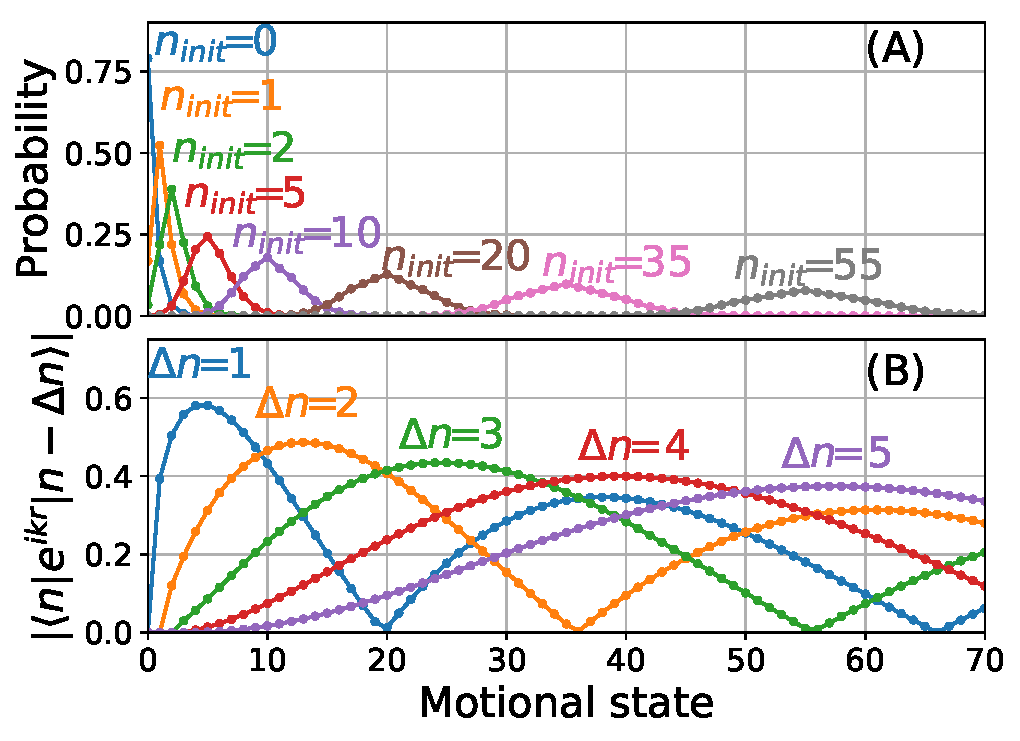
\includegraphics[width=8.5cm]{imgs/fig2_raman_op.pdf}
  \caption{Optical pumping state changing probability and Raman matrix element for axial direction.
    The range plotted covers $95$\% of the initial thermal distribution.
    (A) Axial motional state distribution after one optical pumping cycle
    for different initial $n$. Due to the large Lamb-Dicke parameter,
    there is a high probability of $n$ changing.
    (B) Matrix elements for Raman transition in the axial direction showing deviation from
    $\sqrt{n}$ scaling and multiple minima for different sideband orders.
    ($k$ is the difference in wave vector of the Raman beams,
    $r$ is the coordinate in axial direction).
    \label{f-ld}}
\end{figure}
\begin{figure*}
  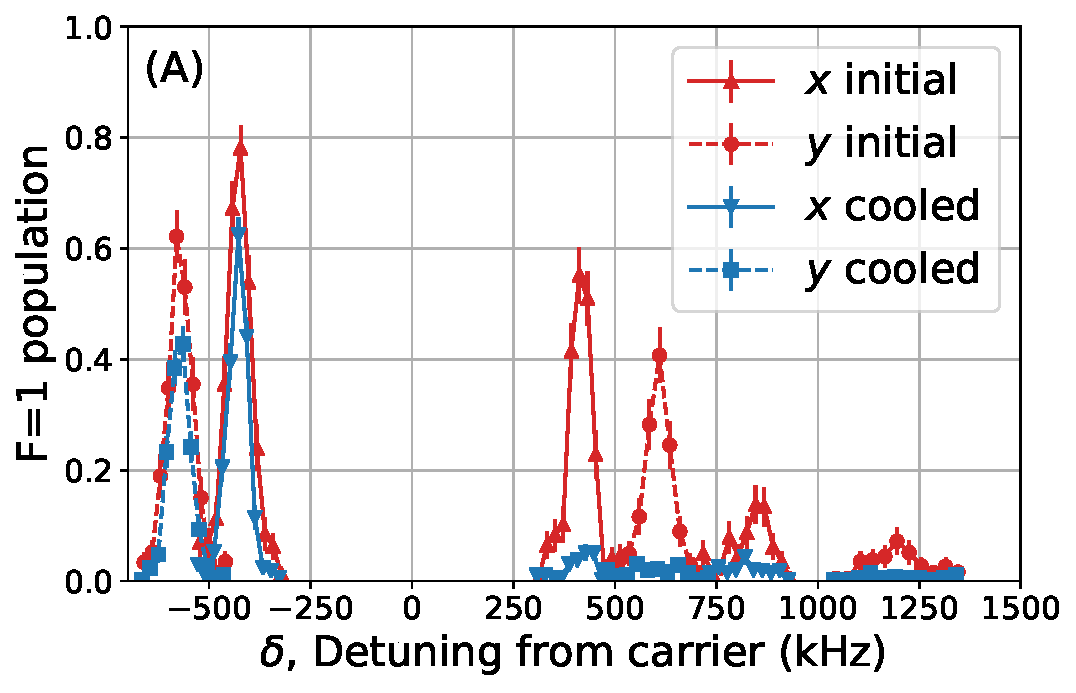
\includegraphics[height=4.2cm]{imgs/spectrum_r.pdf}
  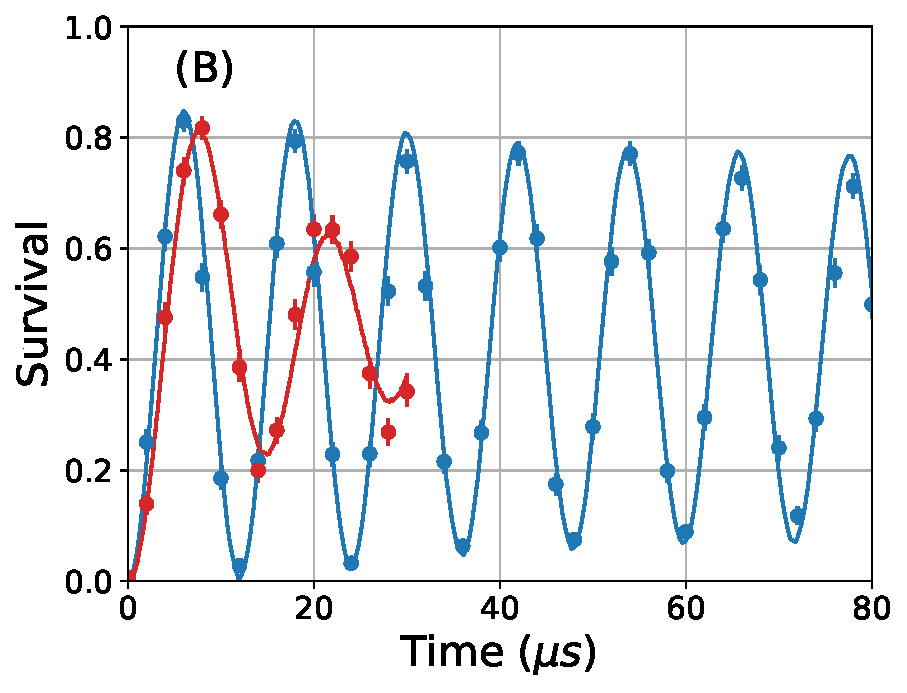
\includegraphics[height=4.2cm]{imgs/rabi_flop_r3_0.pdf}
  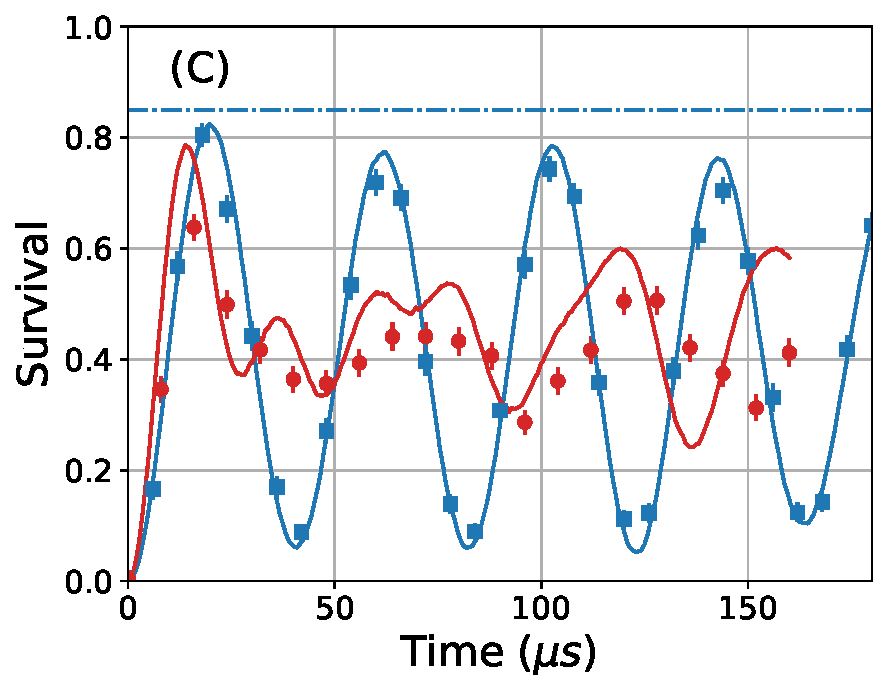
\includegraphics[height=4.2cm]{imgs/rabi_flop_r3_p1.pdf}
  \caption{(A) Radial Raman sideband spectrum of first order heating, first order cooling and
    second order cooling before and after Raman sideband cooling.
    (B,C) Rabi flopping on axis 3 (B) carrier and (C) first order heating sideband
    before (red) and after (blue) cooling.
    Solid lines in (B) and (C) are theoretical calculation of the Rabi flopping.
    The blue lines correspond to a ground state probability of $93$\% after cooling and
    the red lines correspond to a thermal distribution of $70$ $\mu$K before cooling.
    \label{f-radial}}
\end{figure*}
\begin{figure*}
  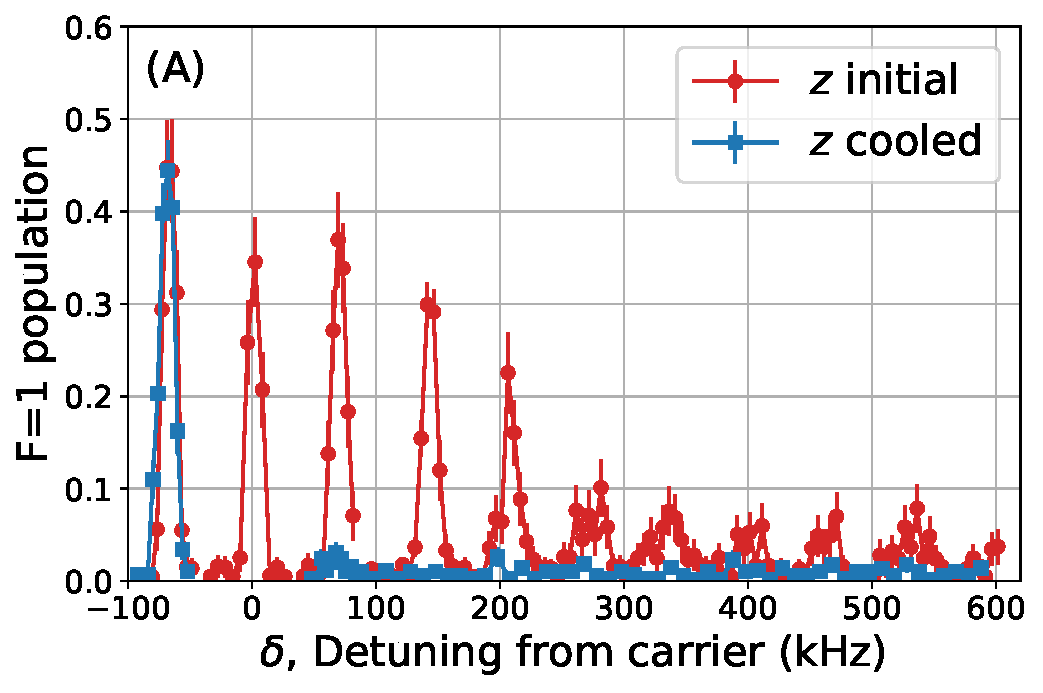
\includegraphics[height=4.2cm]{imgs/spectrum_a1.pdf}
  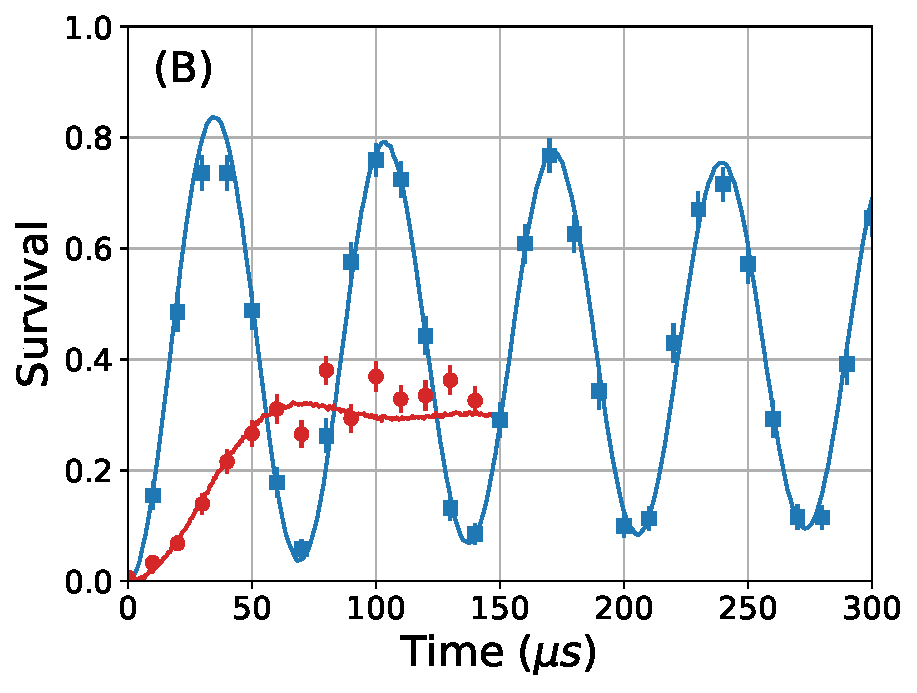
\includegraphics[height=4.2cm]{imgs/rabi_flop_a1_0.pdf}
  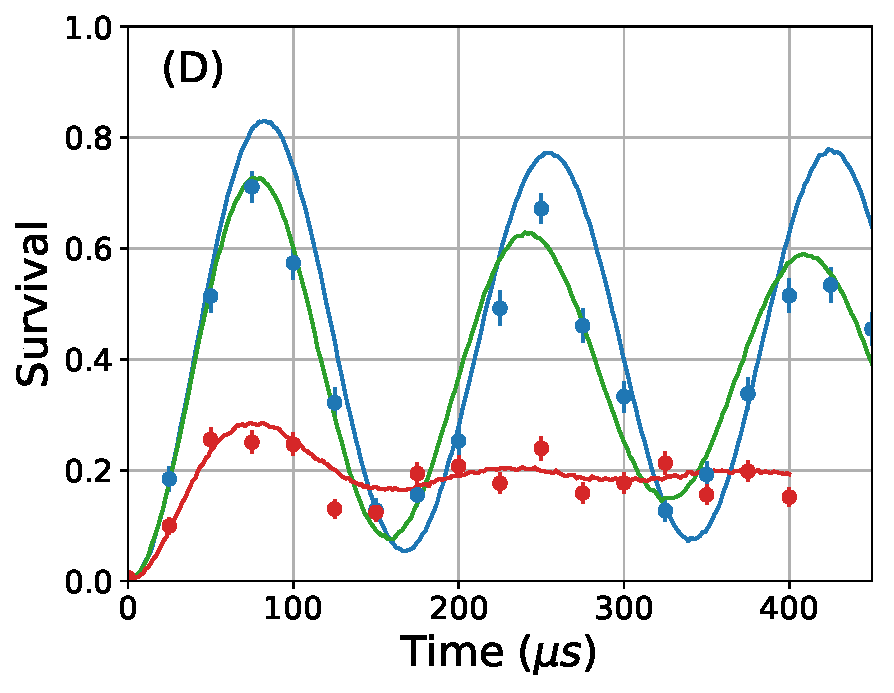
\includegraphics[height=4.2cm]{imgs/rabi_flop_a1_p1.pdf}
  \caption{(A) Axial Raman sideband spectrum from first order heating to eighth order cooling
    before and after Raman sideband cooling.
    The data for the second and higher orders of cooling sidebands are taken with 150 $\mu$s
    pulse time and the rest are taken with 125 $\mu$s pulse time.
    (B,C) Rabi flopping on axial (B) carrier and (C) first order heating sideband
    before (red) and after (blue) cooling.
    Solid lines in (B) and (C) are theoretical calculation of the Rabi flopping.
    The blue and green lines corresponds to a ground state probability of $92$\% after cooling and
    the red lines corresponds to a thermal distribution of $70$ $\mu$K before cooling.
    The blue lines do not take into account the effect of decoherence due to resonance
    fluctuation. By comparing it to the green line in (C), which includes a $3$ kHz fluctuation,
    we can clearly see that this effect is the strongest for the post-cooling data on
    the axial heating sideband where the Rabi frequency is the lowest.
    \label{f-axial}}
\end{figure*}

Systems of trapped neutral atoms assembled from the bottom-up in optical tweezer arrays
are an exciting platform to study quantum information and quantum simulations~\cite{Schlosser2001,Weiss2004,Isenhower2010,Wilk2010,Kaufman2015,Labuhn2016,Murmann2015}.
The inherent single-particle detection and control combined with tunable interactions
are key to implementing neutral atom based quantum logic gates~\cite{Isenhower2010,Wilk2010},
novel quantum phases~\cite{Labuhn2016}, and single-photon switches~\cite{Dayan2008,Tiecke2014}.
Advances in real-time re-arrangement of optical tweezers enable rapid preparation of atoms
in large and complex geometries with high fidelity~\cite{Barredo2016,Endres2016}.
Adding quantum motional control of individual
atoms~\cite{Li2012,Kaufman2012,Thompson2013,Liu2017,Robens2017} enables
efficient coupling of single atoms to photonic crystal cavities~\cite{Thompson2013a},
high-fidelity single qubit gates~\cite{Wang2016},
and studies of the atomic Hong-Ou-Mandel effect~\cite{Kaufman2014}.

Extending optical tweezer array techniques to include polar molecules will open up a large range of
new applications that exploit their many long-lived internal states
and highly tunable interactions~\cite{DeMille2002,Ni2008,Gorshkov2011,Yan2013}.
Molecules could be assembled from atom pairs in the optical tweezer~\cite{Liu2017},
or directly loaded from magneto-optical traps
(MOTs)~\cite{Barry2014,Truppe2017SubDoppler,Anderegg2017}.
For either approach, preparing the constituent atoms or molecules in the lowest motional
quantum state is important for realizing long coherence times in quantum applications.

Preparation of single atoms in the motional ground state has been achieved in optical tweezers~\cite{Kaufman2012,Thompson2013,Liu2017,Robens2017}
 using Raman sideband cooling (RSC)~\cite{Monroe1995,Kerman2000,Han2000}.
However, RSC in these systems has been applied in the Lamb-Dicke (LD) regime, where
the size of the atomic wavefunction is much smaller than the wavelength of light used to address them.
Extending ground state cooling to systems outside the LD regime, such as light atoms or polar molecules, is challenging.
In this letter we demonstrate cooling of single sodium atoms in optical tweezers, initially outside of the LD regime, to the motional ground state.
We achieve a ground state probability of $P_0=77(4)$\% by utilizing cooling of
very high-order sidebands in a carefully optimized cooling sequence.
Our approach is general and opens up ground state cooling for other systems.

Our experiment begins by loading a single sodium atom into an optical tweezer from a MOT
for $250$ ms~\cite{Hutzler2017-LightShifts}, and has an overall repetition rate of $2.5$ Hz.
The tweezer is created by focusing a $700$ nm laser beam through an NA=$0.55$ objective to
create a focused beam with waist $0.7 \mu$m.
With $45$ mW of tweezer power, the trapping frequencies are
$\{\omega_1,\omega_2,\omega_3\}/2\pi = \{69(1), 430(4), 590(5)\}\ \text{\text{kHz}}$.
After attempting to load an atom from the MOT, an image is taken with $1.5$ ms exposure time to determine if it was a success.
The same imaging light is used for polarization gradient cooling (PGC), which
reduces the temperature of the single atom to $70$ $\mu$K,
corresponding to an initial mean motional state along the three different axes of
$\{\bar n_1, \bar n_2, \bar n_3\}=\{21(2),\, 3.4(2),\, 2.5(2)\}$, and therefore initial 3D ground state probability of $P_0=0.3$\%.
A beam with $\sigma^-$-polarization is used to initialize the atom into
the $|F=2, m_F=-2\rangle$ stretched state via optical pumping.
The hyperfine state detection is performed by pushing out atoms in the stretched state with a strong
beam on resonance with the $|F=2, m_F=-2\rangle$ to $|F'=3, m_{F'}=-3\rangle$ transition before
taking the second image to determine if the atom was pushed out.
The state preparation and detection have a combined fidelity of larger than $99$\%.

To further reduce the temperature of the single atom and
to achieve high ground state preparation fidelity, we apply Raman sideband cooling (RSC).
The relevant energy levels, cooling sequence, and Raman beam geometries for our system
are shown in Figure \ref{f-setup}. Briefly, the RSC consists of two steps:
driving a coherent Raman transition while removing motional quanta, followed by resetting the atom's internal state via optical pumping (OP).
RSC is applied repeatedly until the motional ground state is populated with high probability.

Specifically, Raman transitions are driven in Na between the hyperfine states
$|F=2, m_F=-2\rangle$ and  $|F=1, m_F=-1\rangle$ in the presence of a $8.8$ G magnetic field to suppress vector light shifts~\cite{Kaufman2012,Thompson2013}.
Subsequently, an OP/repump pulse brings the atom back to $|F=2, m_F=-2\rangle$
via spontaneous emission.

It is important that the re-pumping step scatter as few photons as possible to minimize heating.  Therefore, we use a $\sigma^-$-polarized laser resonant with the D1 line since the $|F=2, m_F=-2\rangle$ is a dark state in this case \fxnote{cite ion and K39}. Compared to using a D2 repump beam, from which the $|F=2, m_F=-2\rangle$ state could always scatter a photon via the excited $|F=3, m_F=-3\rangle$ state, we find a reduction in the scattering rate of a factor of $130(20)$.

For an atom in motional level $n$, the OP could result in motional-state redistribution
as shown in Fig.~\ref{f-ld}A. The state redistribution probability
is approximately proportional to the effective LD parameter
$\eta^{OP}_{eff}=\sqrt{2n+1}\eta^{OP}$, where $\eta^{OP}=k z_0=k \sqrt{\hbar/2m\omega}$,
$k$ is the wavenumber of the optical pumping beam, $z_0$ is the zero-point wavefunction spread,
$m$ is the mass of the atom, and $\hbar$ is the reduced Planck constant.
Such heating presents a major challenge for efficient cooling of single Na atoms
which feature a light mass and short D-line wavelengths.
For our trap frequencies and beam geometry,
$\{\eta^{OP}_1,\eta^{OP}_2,\eta^{OP}_3\} = \{0.602(5), 0.241(2), 0.206(1)\}$.
Combined with a relatively large PGC temperature gives initial
$\{\eta^{OP}_{1\eff},\eta^{OP}_{2\eff},\eta^{OP}_{3\eff}\} = \{4.0(1), 0.67(2), 0.50(1)\}$.
For the weak axial direction, $(\eta^{OP}_{1\eff})^2>1$ is far outside of the LD regime.
As a result, the average change of motional state per OP step is large,
which creates a large uncertainty on the motional state at the end of a full RSC step, possibly leading to runaway heating.
For example, the average change in motional states over the initial distribution
is $2.4$ in the axial direction, which is significantly greater than $0.89-0.95$
in previous experiments of RSC of Rb and Cs~\cite{Li2012,Kaufman2012,Thompson2013,Liu2017}.

Fortunately, the large LD parameters also provide opportunities to overcome OP heating.
The Raman transitions in our configuration have
$\{\eta^R_{1},\eta^R_{2},\eta^R_{3}\} = \{0.40(1), 0.341(2), 0.291(1)\}$,
which allow strong coupling to higher order sidebands for atoms in higher motional states
as calculated in Figure~\ref{f-ld}B.
To offset heating from OP initially, higher-order Raman cooling sidebands can be utilized
to remove more motional quanta in a single cooling pulse.
Since the coupling strengths of different orders do not reach minima for the same pulse duration,
using multiple orders of cooling sidebands avoids accumulations of population
near the coupling minima.

Taking the large motional-state changing heating and cooling sources into account,
it is not immediately clear that efficient cooling can be achieved.
We therefore use a Monte-Carlo simulation to guide our search and
to find a robust cooling sequence\footnote{See supplemental material}.
In the simulation, we indeed observe a high heating rate due to the large LD parameters
and confirm that cooling with higher-order Raman sidebands can suppress heating.
In particular, we find that instead of cooling on only one sideband order repeatedly,
it is more efficient to alternate the cooling pulses (Fig.~\ref{f-setup}C) between two
neighboring orders for the axial direction and 2nd- and 1st-orders for the radial directions
to minimize the accumulation of the atom in motional states that have zero Raman coupling.
The simulation also indicates that setting the coupling strength of each cooling sideband
to drive a Rabi $\pi$ pulse corresponding to the maximum matrix element motional state
(i.e. the maxima in \ref{f-ld}B) can yield efficient cooling.
The efficiency of cooling on higher-order sidebands diminishes
as the atom approaches the ground state, so the final cooling cycles utilize only the first-order sideband while alternating between the three different axes.

Guided by the simulation results,
we construct our axial cooling sequence by starting at the two highest
observed cooling sidebands (8th- and 7th-orders)
and decreasing the orders after $6$ to $15$ cycles.
This process is repeated until we reach the first order cooling sideband, and most of the
population is in the first few excited states.  We then switch to cooling only on the
first order sideband with two different pulse lengths in order to efficiently cool atoms in the
few remaining motional states.
The radial cooling is performed similarly to the axial cooling with the initial cooling orders being
the 2nd and 1st order and switching to first order only after $20$ to $30$ pulses.
This sequence gives good initial cooling performance, which can then be used to measure experimental
parameters, including the Rabi rates of the Raman beams and optical pumping rates,
in order to optimize the sequence further.

There are two additional important challenges in cooling single sodium atoms.
First, the high initial temperature populates high motional states,
meaning that the atoms sample the anharmonicity of the trap away from the center.
In order to address this, we drive the sidebands with a large Rabi frequency
and short pulses to Fourier broaden the spectrum coverage, and use Blackman pulse envelopes
to avoid unwanted coupling to the carrier and heating sidebands~\cite{Kasevich1992}.
The anharmonicity in the radial directions is calculated to be 1kHz/n, meaning that a
Rabi frequency of at least $15$ kHz is needed to couple to $99$\% population up to $n=15$.
Second, the tweezer trap causes a large AC Stark shift (as large as $300$ MHz)
in the excited state. This creates a large, position-dependent OP detuning
and mixes the excited-state hyperfine levels, which reduces the optical pumping fidelity.
We address this by switching the trapping light at 3 MHz during the whole cooling sequence,
similar to our loading and imaging process~\cite{Hutzler2017-LightShifts},
while leaving OP on with constant intensity.
Due to the large light shift, the OP is effectively off whenever the trap light switches back on.
Since the atom can only be addressed by the optical pumping light when the trap light is off,
the effect of light shifts on OP fidelity is suppressed.

Our final cooling results are shown in Fig.~\ref{f-radial} and \ref{f-axial}.
In total, $1000$ cooling pulses (with a total duration of $100$ ms) are applied along three axes with
cooling beginning on the radial second order.
To characterize the single atom thermal occupation before and after cooling,
we perform Raman sideband thermometry.
For the more tightly confined (non-degenerate) radial directions,
we observe clear first-order heating, first-order cooling,
and second-order cooling sidebands before RSC as is shown in red in Figure \ref{f-radial}A.
After cooling, the first and second order cooling sidebands on both radial axes are suppressed.
It is important to note that the simple sideband thermometry formula,
which predicts the ratio of the cooling and heating sideband heights
to be $\bar n / (\bar n + 1)$~\cite{Monroe1995},
assumes that the coupling strength for different motional states to be proportional to $\sqrt{n}$.
However, outside of the LD regime,
the coupling strength rapidly deviates from this simple scaling rule,
as shown in figure \ref{f-ld}A.  Since the Raman spectroscopy is performed
with relatively large Raman LD parameters $\eta^R$, we cannot use this formula to
measure $\bar n$.
Instead, given the absence of the second order cooling sideband,
we assume \fxnote{[What is the cutoff for the validity of this assumption, and are we below that cutoff?]} that the atoms are cold enough to have stronger coupling to the first order cooling
sideband than the second order, in which case the lower bound of the ground state population
can be computed from the heights of the sidebands by assuming all of the excitations are in the
$n=1$ state. In doing this, we found a ground state population of $90(2)$\%
and $94(3)$\% along the two radial directions.
We also use an independent measurement of Rabi flopping on the carrier (Fig. \ref{f-radial}B)
and first-order heating(Fig. \ref{f-radial}C) sidebands
to verify the ground state population~\cite{Meekhof1996}.
The data is fitted using the same Monte-Carlo simulation we used to simulate the cooling
which yields $89(2)$\% and $92(2)$\% and show good agreement with
the population extracted from the sideband thermometry.
We also extracted the initial temperature before cooling
from the motional-state decohered Rabi flopping to obtain the initial temperature of $70 \mu$K.

For the weaker axial direction, cooling is much more challenging
due to the large $\eta^{OP}_{1eff}\approx 4.0(2)$.
We observe up to 8th-order Raman cooling sidebands initially,
which indicates population in highly-excited motional states.
Nevertheless, our cooling sequence works efficiently as all the cooling sidebands are suppressed
after RSC (Fig.~\ref{f-axial}).
The ground state population calculated using the ratio of first-order sideband heights yields
$92(3)$\%. We also perform Rabi flopping on the carrier(Figure~\ref{f-axial}B)
and extracted a ground state population of $91(2)$\%, in agreement with the other method.
For the first-order heating sideband Rabi flopping (Figure~\ref{f-axial}C),
we observed additional decoherence that is more pronounced due to the slower Rabi frequency.
The decoherence time scale is consistent with magnetic field fluctuations of $1.5$ mG
that we measure independently in the lab, which produces a Zeeman shift of $\sim 3$ kHz.

Combining the axial and radial cooling results,
we have prepared a single Na atom with 3D ground state probability of $77(4)$\%.
We measuring a heating rate of the single atoms in the tweezer to be $0.9$\%/s
due to off-resonant scattering of the trapping light\cite{Grimm2000}.
The ground state preparation fidelity is currently limited by off-resonant scattering
from the Raman beams,
which are measured to be between $3$ to $15$ kHz for the detuning and power we use,
and the resonance shift caused by magnetic field fluctuations.

There is an additional $5$\% loss from finite imaging fidelity and $10$\% loss
from very high-lying initial motional states that are not efficiently cooled by RSC,
but instead off-resonantly heated by the Raman beams.
These give us a $66(3)$\% probability of ground state atom after each successful loading event.
We are planning to improve these by increasing the detuning of the Raman beams,
addressing a wider range of trap anharmonicity by frequency sweeps,
implementing better control of the magnetic field, and optimizing the temperature during imaging.
Another improvement could be to implement grey molasses cooling to achieve
a lower starting temperature before RSC\cite{Colzi2016}.

\fxnote{[The distinction between 77 and 66 percent is confusing, we should discuss it]}

We have shown that despite the difficulty in achieving a low optical cooling temperature
of light mass sodium atoms, reliable three dimensional cooling
with significant ground state population can be achieved by using high-order Raman sidebands
in an optimized cooling sequence.
These techniques are well-suited for a large variety of systems
and open up a route to ground state cooling to other species, including molecules and exotic atoms.

We thank T. Rosenband and J. Hood for valuable discussions.
This work is supported by the NSF through the Harvard-MIT CUA,
the AFOSR Young Investigator Program, the Arnold and Mabel Beckman Foundation,
and the Alfred P. Sloan Foundation.

% Define \eta_R
% Lamb-Dicke parameter square explain
% why not just molecules instead of polar molecules
% entropy
% use different line shape for rabi flopping
% mention axis definitions
% heating from trap -> decrease of ground state procetage (maybe add temprature too)
% Differetial AC starck shift **between excited states and ground states**?
% at the same time, the atom is cooled via PGC instead of "the same imaging light is used to"
% 1 sentence to explain why anisotropy?
% is strobed at 3MHz instead of is switching at...
% Cite Na loading paper in caption?
% Make sure the caption for the before cooling axial rabi flopping mentions decoherence
% Mention after cooling is non-thermal?
% Make it clear that we cool for 6-15 cycles each time before going to the next set of orders in axial

% sm:
% mention the simulation results are 3d
% effect of changing groups.
% mention effects that are included first.

\bibliography{paper}
\end{document}
